\documentclass{article}




\usepackage{fullpage}
\usepackage{nopageno}
\usepackage{amsmath}
\usepackage{amsfonts}
\usepackage{graphicx}
\usepackage{framed}
\usepackage{algorithmic}
\usepackage{xcolor}

\definecolor{dark_red}{rgb}{0.5,0.0,0.0}
\definecolor{dark_green}{rgb}{0.0,0.5,0.0}
\definecolor{dark_blue}{rgb}{0.0,0.0,0.5}
\definecolor{blue}{rgb}{0.0,0.0,1.0}

\newcommand{\dr}[1]{\textcolor{dark_red}{#1}}
\newcommand{\dg}[1]{\textcolor{dark_green}{#1}}
\newcommand{\db}[1]{\textcolor{dark_blue}{#1}}
\newcommand{\blue}[1]{\textcolor{blue}{#1}}



\usepackage{fancyhdr}
%\setlength{\footheight}{15.2pt}
\pagestyle{fancy}
\fancyhead[C]{Wentworth Institute of Technology, MATH2025}
\fancyfoot[C]{Author: Shawn Eastwood}
\renewcommand{\headsep}{25pt}
\renewcommand{\headrulewidth}{1pt}
\renewcommand{\footrulewidth}{1pt}


\begin{document}

\section*{Triple Integrals}


\begin{tabular}{cc}
\parbox{0.5\textwidth}{
Given a function \(f(\mathbf{q})\) whose domain is a set of points in 3D space, the {\bf triple integral} over the 3D region \(\Omega \subseteq \mathbb{R}^3\) is defined by the following Riemann sum:

Let \(N\) denote a large integer. Partition the region \(\Omega\) into a set of \(N\) tiny regions as depicted to the right. For each \(i = 1, 2, ..., N\), the \(i^{\text{th}}\) section has a volume of \(\Delta V_i\) and contains the ``representative" point \(\mathbf{q}_i^*\). The triple integral of \(f(\mathbf{q})\) over the region \(\Omega\) is the limit: 

\[\iiint_{\Omega} f(\mathbf{q})dV = \lim_{N \rightarrow +\infty} \sum_{i=1}^N f(\mathbf{q}_i^*)\Delta V_i\]

} & \parbox{0.5\textwidth}{
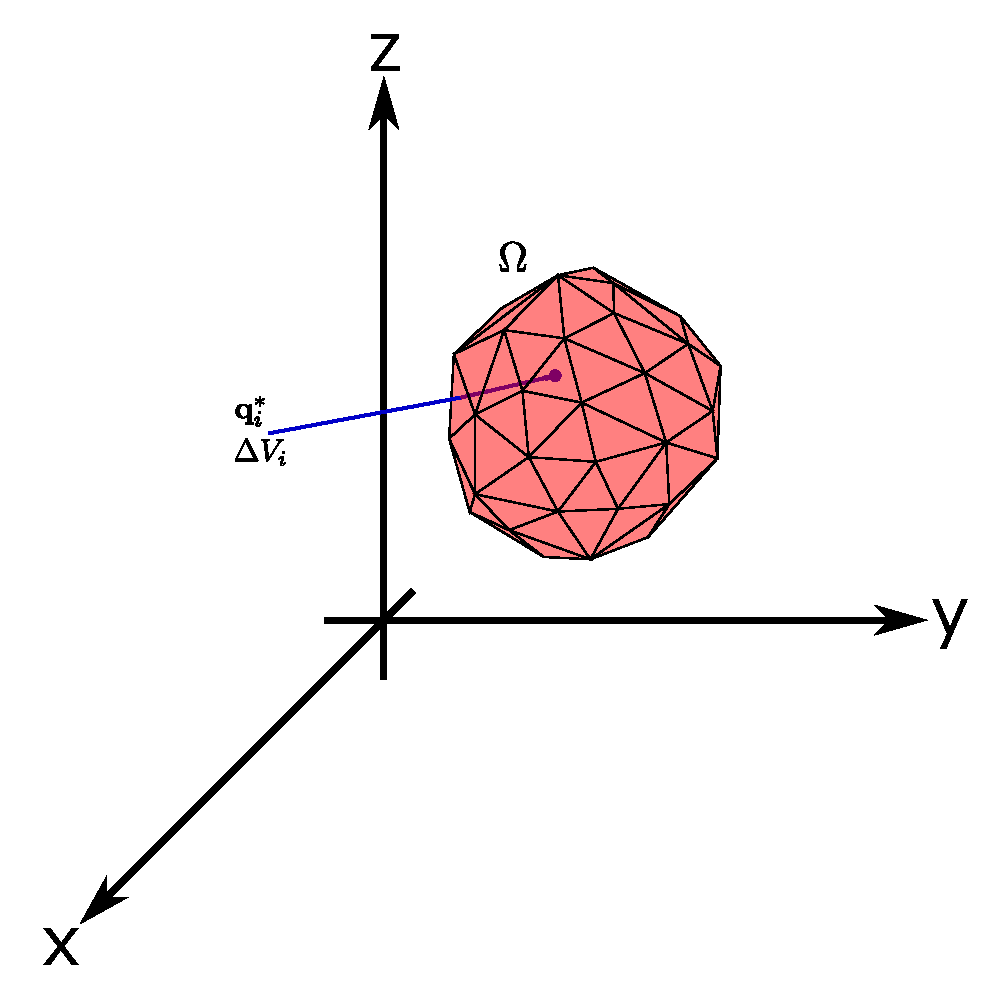
\includegraphics[width = 0.5\textwidth]{triple_integral_riemann_sum}
}
\end{tabular}

If the integrand \(f(\mathbf{q})\) is \(1\), then the triple integral evaluates to: 
\[\iiint_{\Omega} dV = \lim_{N \rightarrow +\infty} \sum_{i=1}^N \Delta V_i = \text{volume of \(\Omega\)}\]



\section*{Triple integrals using Cartesian coordinates}

There are several approaches to quantifying 3D regions using Cartesian coordinates. All approaches have the following pattern. The bounds on one of the coordinates are fixed constant values. The bounds on a second coordinate may only depend on the first coordinate, and lastly the bounds on the final coordinate may only depend on the first two coordinates. For example, if: 
\[\Omega = \{(x,y,z) | a_L \leq x \leq a_U \;\&\; b_L(x) \leq y \leq b_U(x) \;\&\; c_L(x,y) \leq z \leq c_U(x,y)\}\]
then the lower and upper bounds of \(x\) are fixed to \(a_L\) and \(a_U\) respectively. The lower and upper bounds on \(y\) depend only on \(x\), and are respectively \(b_L(x)\) and \(b_U(x)\). Lastly the lower and upper bounds on \(z\) depend only on \(x\) and \(y\), respectively \(c_L(x,y)\) and \(c_U(x,y)\). 

There are 6 possible orderings:
\[\Omega = \{(x,y,z) | a_L \leq x \leq a_U \;\&\; b_L(x) \leq y \leq b_U(x) \;\&\; c_L(x,y) \leq z \leq c_U(x,y)\}\]
\[\Omega = \{(x,y,z) | a_L \leq x \leq a_U \;\&\; c_L(x,z) \leq y \leq c_U(x,z) \;\&\; b_L(x) \leq z \leq b_U(x)\}\]
\[\Omega = \{(x,y,z) | b_L(y) \leq x \leq b_U(y) \;\&\; a_L \leq y \leq a_U \;\&\; c_L(x,y) \leq z \leq c_U(x,y)\}\]
\[\Omega = \{(x,y,z) | c_L(y,z) \leq x \leq c_U(y,z) \;\&\; a_L \leq y \leq a_U \;\&\; b_L(y) \leq z \leq b_U(y)\}\]
\[\Omega = \{(x,y,z) | b_L(z) \leq x \leq b_U(z) \;\&\; c_L(x,z) \leq y \leq c_U(x,z) \;\&\; a_L \leq z \leq a_U\}\]
\[\Omega = \{(x,y,z) | c_L(y,z) \leq x \leq c_U(y,z) \;\&\; b_L(z) \leq y \leq b_U(z) \;\&\; a_L \leq z \leq a_U\}\]

Using Cartesian coordinates, the triple integral \(\iiint_{\Omega} f(x,y,z)dV\) where
\[\Omega = \{(x,y,z) | a_L \leq x \leq a_U \;\&\; b_L(x) \leq y \leq b_U(x) \;\&\; c_L(x,y) \leq z \leq c_U(x,y)\}\]
will now be evaluated using a nested series of 3 integrals. To establish the single integral expression for \(\iiint_{\Omega} f(x,y,z)dV\), the region \(\Omega\) will be sliced into a series of \(N\) slices where \(N\) is a large number, as depicted in the image below. For each \(i = 1, 2, ..., N\), the width of the \(i^{\text{th}}\) slice is \(\Delta x_i\), and \(x_i^*\) is a ``representative" \(x\) value from the \(i^{\text{th}}\) slice. 
Now for each slice, further partition the slice into a series of \(M\) columns where \(M\) is a large number, as depicted in the image below. For each \(i = 1, 2, ..., N\) and for each \(j = 1, 2, ..., M\), the width of the \(j^{\text{th}}\) column in the \(i^{\text{th}}\) slice is \(\Delta y_{(i,j)}\), and \(y_{(i,j)}^*\) is a ``representative" \(y\) value from the \(j^{\text{th}}\) column in the \(i^{\text{th}}\) slice. 
Now for each column, further partition the column into a series of \(L\) bricks where \(L\) is a large number, as depicted in the image below. For each \(i = 1, 2, ..., N\), for each \(j = 1, 2, ..., M\), and for each \(k = 1, 2, ..., L\) the height of the \(k^{\text{th}}\) brick in the \(j^{\text{th}}\) column in the \(i^{\text{th}}\) slice is \(\Delta z_{(i,j,k)}\), and \(z_{(i,j,k)}^*\) is a ``representative" \(z\) value from the \(k^{\text{th}}\) brick in the \(j^{\text{th}}\) column in the \(i^{\text{th}}\) slice. The volume of the \(k^{\text{th}}\) brick in the \(j^{\text{th}}\) column in the \(i^{\text{th}}\) slice is \(\Delta V_{(i,j,k)} = \Delta x_i \Delta y_{(i,j)} \Delta z_{(i,j,k)}\).   

\begin{center}
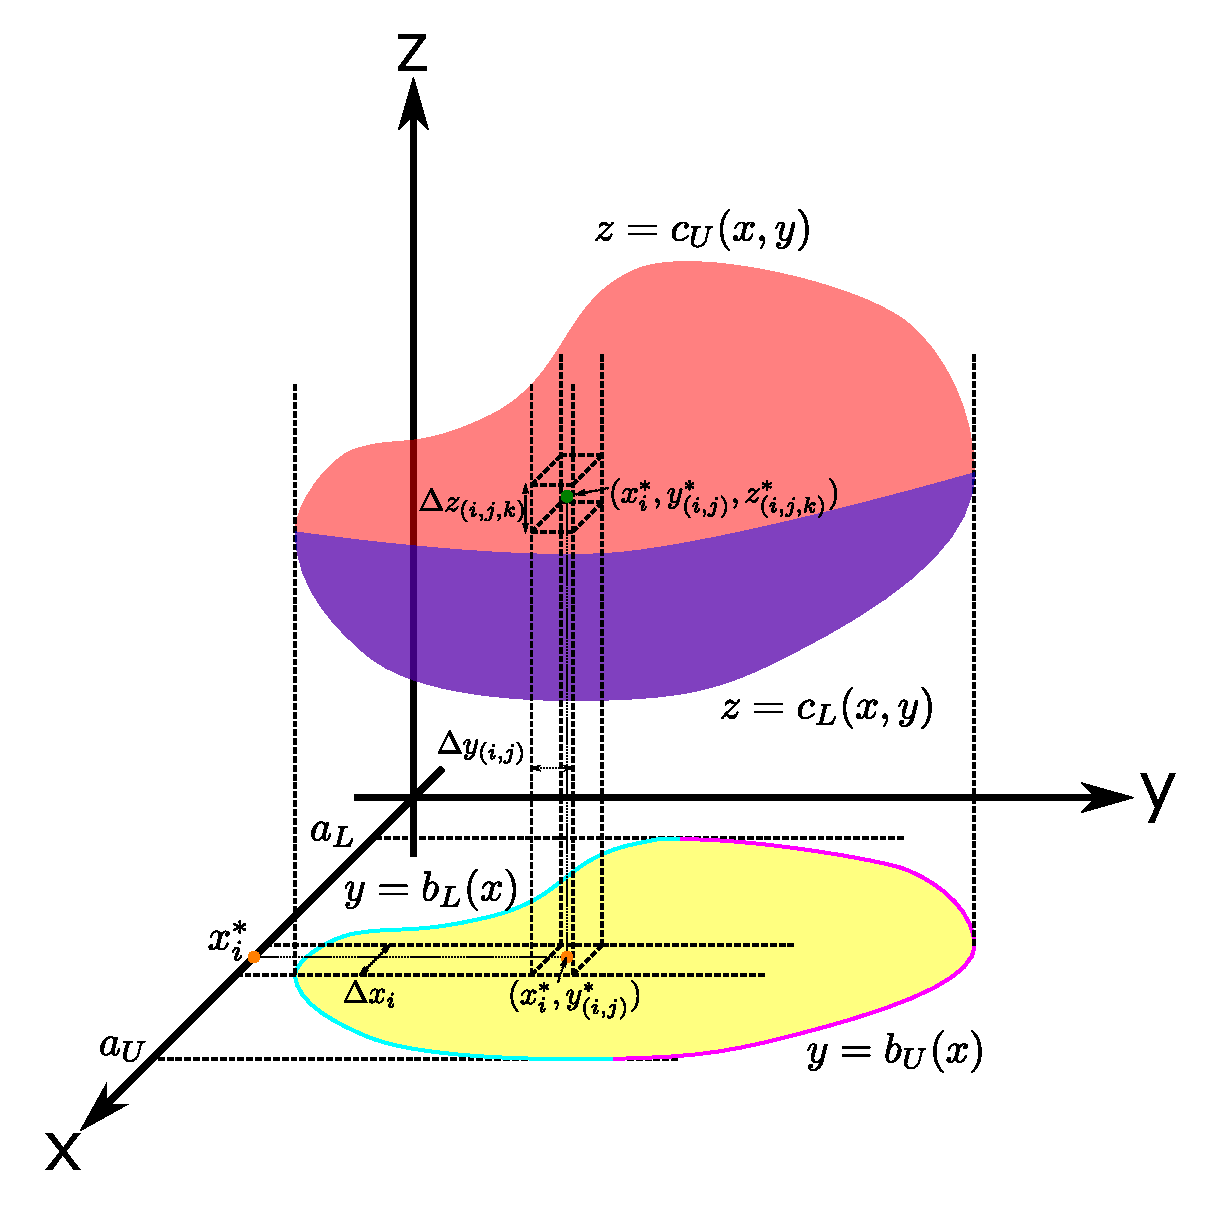
\includegraphics[width = 0.75\textwidth]{cartesian_riemann_sum}
\end{center}

Evaluating the Riemann sum gives:

\begin{align*}
\iiint_{\Omega} f(x,y,z)dV = & \lim_{N \rightarrow +\infty} \lim_{M \rightarrow +\infty} \lim_{L \rightarrow +\infty} \sum_{i=1}^N \sum_{j = 1}^M \sum_{k = 1}^L f(x_i^*, y_{(i,j)}^*, z_{(i,j,k)}^*) \Delta V_{(i,j,k)} \\ 
= & \lim_{N \rightarrow +\infty} \lim_{M \rightarrow +\infty} \lim_{L \rightarrow +\infty} \sum_{i=1}^N \sum_{j = 1}^M \sum_{k = 1}^L f(x_i^*, y_{(i,j)}^*, z_{(i,j,k)}^*) (\Delta x_i \Delta y_{(i,j)} \Delta z_{(i,j,k)}) \\ 
= & \lim_{N \rightarrow +\infty} \sum_{i=1}^N \left(\lim_{M \rightarrow +\infty} \sum_{j = 1}^M \left(\lim_{L \rightarrow +\infty} \sum_{k = 1}^L f(x_i^*, y_{(i,j)}^*, z_{(i,j,k)}^*) \Delta z_{(i,j,k)} \right)\Delta y_{(i,j)}\right)\Delta x_i \\
= & \lim_{N \rightarrow +\infty} \sum_{i=1}^N \left(\lim_{M \rightarrow +\infty} \sum_{j = 1}^M \left(\int_{z = c_L(x_i^*, y_{(i,j)}^*)}^{c_U(x_i^*, y_{(i,j)}^*)} f(x_i^*, y_{(i,j)}^*, z) dz \right)\Delta y_{(i,j)}\right)\Delta x_i \\   
= & \lim_{N \rightarrow +\infty} \sum_{i=1}^N \left(\int_{y = b_L(x_i^*)}^{b_U(x_i^*)} \left(\int_{z = c_L(x_i^*, y)}^{c_U(x_i^*, y)} f(x_i^*, y, z) dz \right) dy \right)\Delta x_i \\   
= & \int_{x = a_L}^{a_U} \left(\int_{y = b_L(x)}^{b_U(x)} \left(\int_{z = c_L(x, y)}^{c_U(x, y)} f(x, y, z) dz \right) dy \right) dx
\end{align*}

Therefore:
\[\iiint_{\Omega} f(x,y,z)dV = \int_{x = a_L}^{a_U} \left(\int_{y = b_L(x)}^{b_U(x)} \left(\int_{z = c_L(x, y)}^{c_U(x, y)} f(x, y, z) dz \right) dy \right) dx\]

Similar formulas exist for other orderings of the \(x\), \(y\), and \(z\) coordinates. In general, the variable with the fixed bounds is the integration variable of the outermost integral. The variable whose bounds may only depend on the variable with the fixed bounds is the integration variable of the middle integral. The remaining variable is the integration variable of the innermost integral. It is important to note that {\bf a variable of integration cannot exist outside of the integrand of its respective integral}. An integral over the variable \(x\) cannot incorporate \(x\) in the expressions for its bounds, nor can \(x\) exist outside of the integral itself.

\vspace{5mm}

\textbf{Examples:}

\begin{itemize}
%%%%%%%%%%%%%%%%
\item Let: 
\[\Omega = \left\{(x,y,z) \middle| -\pi \leq x \leq \pi \;\&\; 0 \leq y \leq 2\pi \;\&\; -1 \leq z \leq 3 \right\}\] 
The triple integral \(\iiint_{\Omega} z\cos\left(\frac{x+y}{2}\right) dV\) is sought. Note that the bounds on \(x\), \(y\), and \(z\) are all fixed, so any of these variables can be the outermost, middle, or inner variables of integration. There is no preferred ordering. Choosing \(x\) to be the outermost variable, and \(z\) to be the innermost variable gives:
\begin{align*}
& \iiint_{\Omega} z\cos\left(\frac{x+y}{2}\right) dV = \int_{x = -\pi}^{\pi} \left(\int_{y = 0}^{2\pi} \left(\int_{z = -1}^3 z\cos\left(\frac{x+y}{2}\right)dz\right)dy\right)dx \\
& = \int_{x = -\pi}^{\pi} \left(\int_{y = 0}^{2\pi} \frac{1}{2}z^2\cos\left(\frac{x+y}{2}\right)\Bigg|_{z = -1}^3 dy\right)dx 
= \int_{x = -\pi}^{\pi} \left(\int_{y = 0}^{2\pi} 4\cos\left(\frac{x+y}{2}\right) dy\right)dx \\  
& = \int_{x = -\pi}^{\pi} 8\sin\left(\frac{x+y}{2}\right)\Bigg|_{y = 0}^{2\pi}dx 
= \int_{x = -\pi}^{\pi} \left(8\sin\left(\frac{x}{2} + \pi\right) - 8\sin\left(\frac{x}{2}\right)\right)dx \\
& = \int_{x = -\pi}^{\pi} \left(-8\sin\left(\frac{x}{2}\right) - 8\sin\left(\frac{x}{2}\right)\right)dx 
= \int_{x = -\pi}^{\pi} -16\sin\left(\frac{x}{2}\right)dx 
= 32\cos\left(\frac{x}{2}\right)\Bigg|_{x = -\pi}^{\pi} \\
& = 32\cos\left(\frac{\pi}{2}\right) - 32\cos\left(-\frac{\pi}{2}\right) 
= 0 - 0 = 0
\end{align*}



%%%%%%%%%%%%%%%%
\item Let: 
\[\Omega = \left\{(x,y,z) \middle| 0 \leq x \leq y \;\&\; 1 \leq y \leq 2 \;\&\; 0 \leq z \leq \frac{1}{y} \right\}\] 
The triple integral \(\iiint_{\Omega} x^3 y z^2 dV\) is sought. The bounds on \(y\) are fixed, so \(y\) is the outermost variable of integration. The bounds on \(x\) and \(z\) do not depend on each other, only on \(y\), so any of these variables can be the middle or inner variables of integration. There is no preferred ordering amongst \(x\) and \(z\). Choosing \(x\) to be the middle variable, and \(z\) to be the innermost variable gives:
\begin{align*}
& \iiint_{\Omega} x^3 y z^2 dV 
= \int_{y = 1}^2 \left(\int_{x = 0}^y \left(\int_{z = 0}^{1/y} x^3 y z^2 dz\right)dx\right)dy 
= \int_{y = 1}^2 \left(\int_{x = 0}^y \frac{1}{3} x^3 y z^3 \bigg|_{z = 0}^{1/y} dx\right)dy \\  
& = \int_{y = 1}^2 \left(\int_{x = 0}^y \frac{x^3}{3y^2} dx\right)dy 
= \int_{y = 1}^2 \frac{x^4}{12y^2}\bigg|_{x = 0}^y dy 
= \int_{y = 1}^2 \frac{y^2}{12} dy 
= \frac{y^3}{36}\bigg|_{y = 1}^2 
= \frac{7}{36}
\end{align*}



%%%%%%%%%%%%%%%%
\item Let:
\[\Omega = \left\{(x,y,z) \middle| 0 \leq x \leq 4 \;\&\; 0 \leq y \leq \frac{3}{4}x \;\&\; 0 \leq z \leq (2/3)y \right\}\]  
The triple integral \(\iiint_{\Omega} (x + y + z)dV\) is sought. The bounds on \(x\) are fixed, so \(x\) is the outermost variable of integration. The bounds on \(y\) depend only on \(x\), so \(y\) is the middle variable of integration. \(z\) is the innermost variable of integration.   
\begin{align*}
& \iiint_{\Omega} (x + y + z)dV 
= \int_{x = 0}^4 \left(\int_{y = 0}^{\frac{3}{4}x} \left(\int_{z = 0}^{\frac{2}{3}y} (x + y + z)dz\right)dy\right)dx \\ 
& = \int_{x = 0}^4 \left(\int_{y = 0}^{\frac{3}{4}x} (xz + yz + \frac{1}{2}z^2)\Big|_{z = 0}^{\frac{2}{3}y}dy\right)dx 
= \int_{x = 0}^4 \left(\int_{y = 0}^{\frac{3}{4}x} (\frac{2}{3}xy + \frac{2}{3}y^2 + \frac{2}{9}y^2)dy\right)dx \\  
& = \int_{x = 0}^4 \left(\int_{y = 0}^{\frac{3}{4}x} (\frac{2}{3}xy + \frac{8}{9}y^2)dy\right)dx  
= \int_{x = 0}^4 (\frac{1}{3}xy^2 + \frac{8}{27}y^3)\Big|_{y = 0}^{\frac{3}{4}x} dx 
= \int_{x = 0}^4 (\frac{3}{16}x^3 + \frac{1}{8}x^3) dx \\
& = \int_{x = 0}^4 \frac{5}{16}x^3 dx 
= \frac{5}{64}x^4\Big|_{x = 0}^4  
= 20
\end{align*}


%%%%%%%%%%%%%%%%
\item Let:
\[\Omega = \left\{(x,y,z) \middle| 0 \leq x \leq 3z \;\&\; 0 \leq y \leq 1 \;\&\; 0 \leq z \leq 2y \right\}\]  
The triple integral \(\iiint_{\Omega} (x + y + z)dV\) is sought. The bounds on \(y\) are fixed, so \(y\) is the outermost variable of integration. The bounds on \(z\) depend only on \(y\), so \(z\) is the middle variable of integration. \(x\) is the innermost variable of integration.   
\begin{align*}
& \iiint_{\Omega} (x + y + z)dV  
= \int_{y = 0}^1 \left(\int_{z = 0}^{2y} \left(\int_{x = 0}^{3z} (x + y + z)dx\right)dz\right)dy \\ 
& = \int_{y = 0}^1 \left(\int_{z = 0}^{2y} (\frac{1}{2}x^2 + xy + xz)\Big|_{x = 0}^{3z} dz\right)dy    
= \int_{y = 0}^1 \left(\int_{z = 0}^{2y} (\frac{9}{2}z^2 + 3yz + 3z^2) dz\right)dy \\   
& = \int_{y = 0}^1 \left(\int_{z = 0}^{2y} (\frac{15}{2}z^2 + 3yz) dz\right)dy 
= \int_{y = 0}^1 (\frac{5}{2}z^3 + \frac{3}{2}yz^2)\Big|_{z = 0}^{2y} dy  
= \int_{y = 0}^1 (20y^3 + 6y^3) dy \\   
& = \int_{y = 0}^1 26y^3 dy 
= \frac{13}{2}y^4\Big|_{y = 0}^1 
= \frac{13}{2} 
\end{align*}


\end{itemize}




\section*{Triple integrals using Cylindrical coordinates}

\begin{tabular}{cc}
\parbox{0.5\textwidth}{
{\bf Cylindrical coordinates} are a generalization of Polar coordinates to 3 dimensions. Cylindrical coordinates are to Polar coordinates what 3D Cartesian coordinates are to 2D Cartesian coordinates. A point is described by the triple of numbers \((r,\theta,z)\). The pair \((r, \theta)\) are the Polar coordinates of the projection of the point onto the \(xy\)-plane, while \(z\) is simply the \(z\) coordinate. This is illustrated on the right.
} & \parbox{0.5\textwidth}{
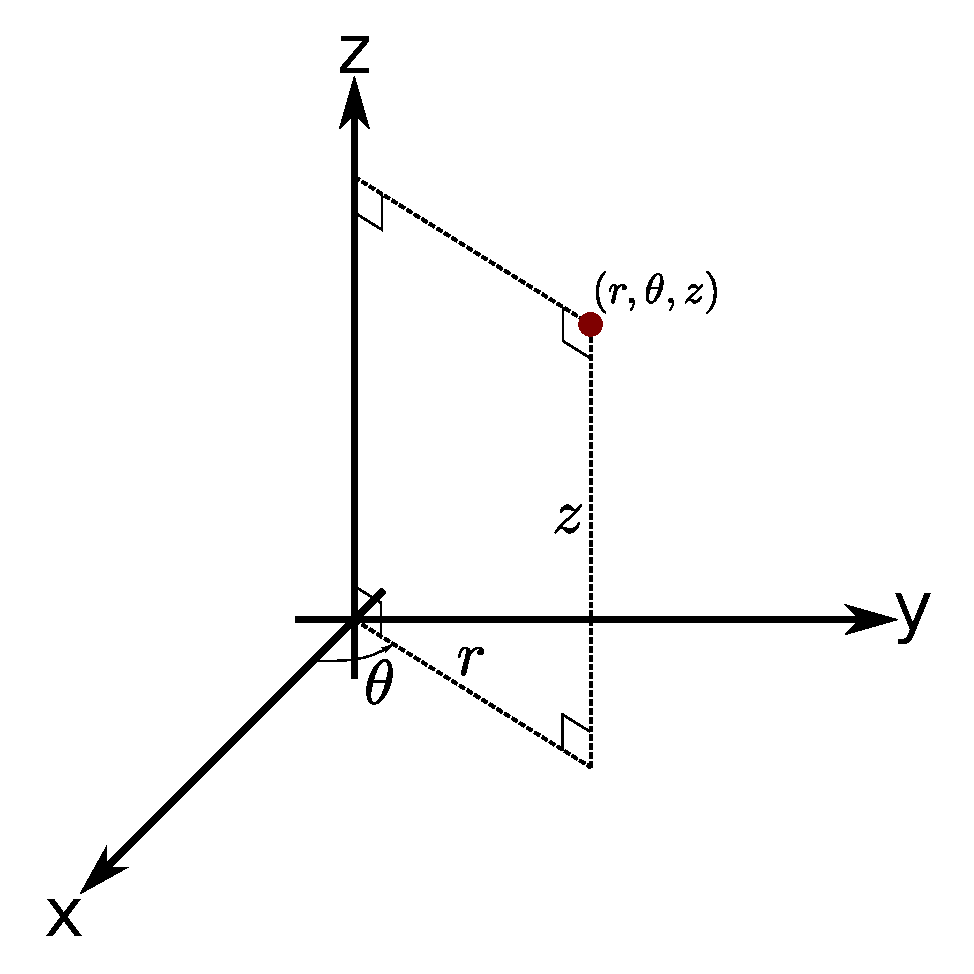
\includegraphics[width = 0.5\textwidth]{cylindrical_coordinates}
}
\end{tabular}

\begin{tabular}{cc}
\parbox{0.5\textwidth}{
Similar to double integrals using Polar coordinates, when converting a triple integral to a triple nested integral, the integrand must be multiplied by \(r\). This is because while the volume of an infinitesimal rectangular prism is \(\Delta x \Delta y \Delta z\), the volume of a ``cylindrical box", shown on the right, is actually \(r^* \Delta r \Delta \theta \Delta z\), where \(r^*\) is a ``representative" value of \(r\) from inside the box. This follows from the fact that the ``dimensions" of the cylindrical box parallel to the \(r\), \(\theta\), and \(z\) directions are respectively approximately \(\Delta r\), \(r^* \Delta\theta\), and \(\Delta z\) so
\[\Delta V = (\Delta r)(r^* \Delta\theta)(\Delta z) = r^* \Delta r \Delta\theta \Delta z\]
} & \parbox{0.5\textwidth}{
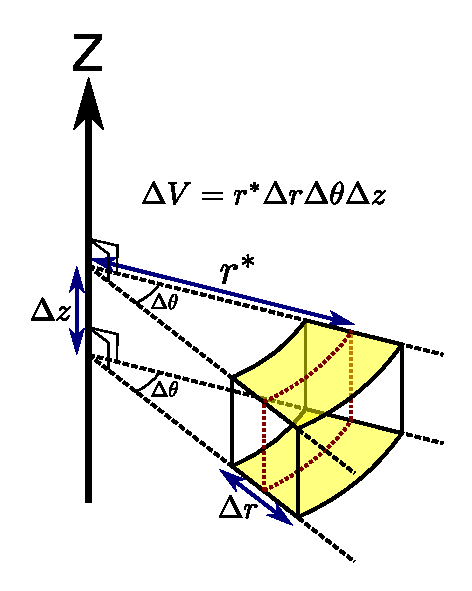
\includegraphics[width = 0.5\textwidth]{cylindrical_box}
}
\end{tabular}

\textbf{Examples:}

\begin{itemize}
%%%%%%%%%%%%%%%%%%%%%%%%%%%%
\item Let:
\[\Omega = \left\{(r,\theta,z) \middle| 0 \leq r \leq 2 \;\&\; 0 \leq \theta \leq 2\pi \;\&\; 0 \leq z \leq 3 - \frac{3}{2}r \right\}\]
The triple integral \(\iiint_{\Omega}z \cdot dV\) is sought. The bounds on \(r\) are fixed, and the bounds on \(\theta\) are fixed, so either \(r\) or \(\theta\) can be the outermost variable of integration, while the other variable is the middle variable of integration. \(z\) will be the innermost variable of integration. When the triple integral becomes a triple nested integral, note that the integrand is multiplied by \(r\).
\begin{align*}
& \iiint_{\Omega} z \cdot dV 
= \int_{\theta = 0}^{2\pi} \left(\int_{r = 0}^2 \left(\int_{z = 0}^{3 - (3/2)r} z \cdot r \cdot dz\right)dr\right)d\theta \\ 
& = \int_{\theta = 0}^{2\pi} \left(\int_{r = 0}^2 \left(\frac{1}{2}r \cdot z^2\Big|_{z = 0}^{3 - (3/2)r}\right)dr\right)d\theta 
= \int_{\theta = 0}^{2\pi} \left(\int_{r = 0}^2 \left(\frac{9}{2}r - \frac{9}{2}r^2 + \frac{9}{8}r^3\right)dr\right)d\theta \\
& = \int_{\theta = 0}^{2\pi} \left(\frac{9}{4}r^2 - \frac{3}{2}r^3 + \frac{9}{32}r^4\right)\bigg|_{r=0}^2 d\theta 
= \int_{\theta = 0}^{2\pi} \left(9 - 12 + \frac{9}{2}\right)d\theta 
= \int_{\theta = 0}^{2\pi} \frac{3}{2}d\theta 
= 3\pi
\end{align*}
 

%%%%%%%%%%%%%%%%%%%%%%%%%%%%
\item Let:
\[\Omega = \left\{(r,\theta,z) \middle| 0 \leq r \leq 2\cos\theta \;\&\; -\frac{\pi}{2} \leq \theta \leq \frac{\pi}{2} \;\&\; 0 \leq z \leq r\cos\theta \right\}\]
The triple integral \(\iiint_{\Omega} (1 + r\sin\theta)dV\) is sought. The bounds on \(\theta\) are fixed, so \(\theta\) is the outermost variable of integration. The bounds on \(r\) depend only on \(\theta\), so \(r\) is the middle variable of integration. \(z\) is the innermost variable of integration. When the triple integral becomes a triple nested integral, note that the integrand is multiplied by \(r\).
\begin{align*}
& \iiint_{\Omega} (1 + r\sin\theta) dV 
= \int_{\theta = -\pi/2}^{\pi/2} \left(\int_{r = 0}^{2\cos\theta} \left(\int_{z = 0}^{r\cos\theta} (1 + r\sin\theta) \cdot r \cdot dz\right)dr\right)d\theta \\
& = \int_{\theta = -\pi/2}^{\pi/2} \left(\int_{r = 0}^{2\cos\theta} (r + r^2 \sin\theta)z \Big|_{z = 0}^{r\cos\theta} dr\right)d\theta 
= \int_{\theta = -\pi/2}^{\pi/2} \left(\int_{r = 0}^{2\cos\theta} (r^2 + r^3\sin\theta)\cos\theta dr\right)d\theta \\  
& = \int_{\theta = -\pi/2}^{\pi/2} \left( \frac{1}{3}r^3 + \frac{1}{4}r^4\sin\theta \right)\cos\theta \Big|_{r = 0}^{2\cos\theta} d\theta  
= \int_{\theta = -\pi/2}^{\pi/2} \left( \frac{8}{3}\cos^3 \theta + 4\cos^4\theta \sin\theta \right)\cos\theta d\theta \\   
& = \frac{8}{3}\int_{\theta = -\pi/2}^{\pi/2} \cos^4\theta d\theta + 4\int_{\theta = -\pi/2}^{\pi/2} \cos^5\theta \sin\theta d\theta 
\end{align*}
\begin{align*}
& = \frac{8}{3}\int_{\theta = -\pi/2}^{\pi/2} \left(\frac{1 + \cos(2\theta)}{2}\right)^2 d\theta - \frac{2}{3}\cos^6\theta\Big|_{\theta = -\pi/2}^{\pi/2} 
= \frac{2}{3}\int_{\theta = -\pi/2}^{\pi/2} (1 + 2\cos(2\theta) + \cos^2(2\theta))d\theta \\
& = \frac{2}{3}\left((\theta + \sin(2\theta))\Big|_{\theta = -\pi/2}^{\pi/2} + \int_{\theta = -\pi/2}^{\pi/2} \frac{1 + \cos(4\theta)}{2}d\theta\right) \\
& = \frac{2}{3}\left(\pi + (\frac{1}{2}\theta + \frac{1}{8}\sin(4\theta))\Big|_{\theta = -\pi/2}^{\pi/2}\right) 
= \frac{2}{3}\left(\pi + \frac{1}{2}\pi\right) 
= \pi
\end{align*}

\end{itemize}



\section*{Triple integrals using Spherical coordinates}

\begin{tabular}{cc}
\parbox{0.5\textwidth}{
{\bf Spherical coordinates} are a further generalization of Polar coordinates to 3 dimensions. Unlike cylindrical coordinates where the third coordinate is simply the \(z\) from Cartesian coordinates, the third coordinate is also an angle. A point is described by the triple of numbers \((\rho,\theta,\phi)\). \(\rho\) is the point's distance from the origin. \(\theta\) is the ``azimuth", which is essentially the longitude coordinate: the counterclockwise angle that the projection of the position vector onto the \(xy\) plane makes with the positive \(x\) axis. Lastly \(\phi\) is the angle with the positive \(z\) axis. This is illustrated on the right.
} & \parbox{0.5\textwidth}{
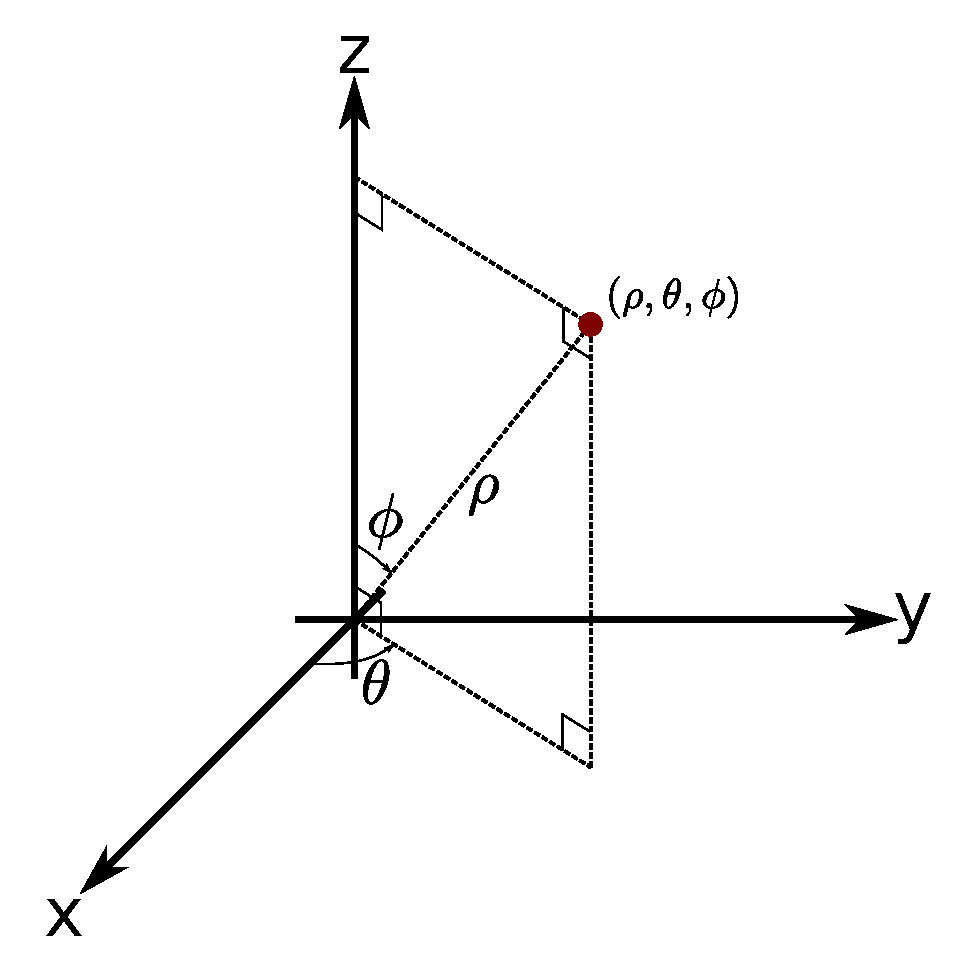
\includegraphics[width = 0.5\textwidth]{spherical_coordinates}
}
\end{tabular}

\begin{tabular}{cc}
\parbox{0.5\textwidth}{
In contrast to cylindrical coordinates, when converting a triple integral to a triple nested integral in spherical coordinates, the integrand must be multiplied by \(\rho^2\sin\phi\). This is because while the volume of an infinitesimal cylindrical box is \(r^* \Delta r \Delta \theta \Delta z\), the volume of a ``spherical box", shown on the right, is actually \((\rho^*)^2 (\sin\phi^*) \Delta\rho \Delta \theta \Delta \phi\), where \(\rho^*\) is a ``representative" value of \(\rho\) from inside the box, and \(\phi^*\) is a ``representative" value of \(\phi\) from inside the box. This follows from the fact that the ``dimensions" of the spherical box parallel to the \(\rho\), \(\theta\), and \(\phi\) directions are respectively approximately \(\Delta \rho\); ~ \(\rho^*\sin\phi^* \Delta\theta\); ~ and \(\rho^* \Delta \phi\) so
\[\Delta V = (\Delta \rho)(\rho^*\sin\phi^* \Delta\theta)(\rho^* \Delta \phi) = (\rho^*)^2 (\sin\phi^*) \Delta\rho \Delta \theta \Delta \phi\]
} & \parbox{0.5\textwidth}{
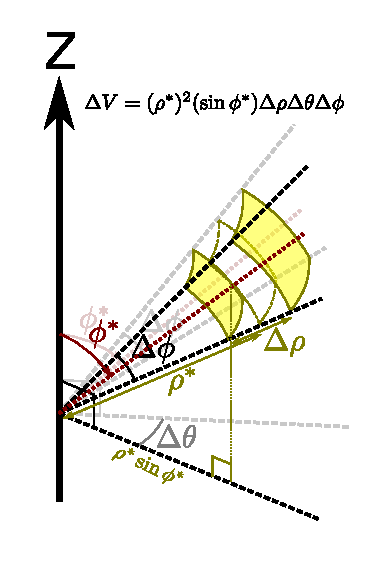
\includegraphics[width = 0.5\textwidth]{spherical_box}
}
\end{tabular}

\textbf{Examples:}

\begin{itemize}
%%%%%%%%%%%%%%%%%%%%%%%%%%%%
\item Let:
\[\Omega = \{(\rho,\theta,\phi) | 0 \leq \rho \leq a \;\&\; 0 \leq \theta \leq 2\pi \;\&\; 0 \leq \phi \leq \pi\}\]
where \(a\) is a positive constant. \(\Omega\) is a sphere with a radius of \(a\) that is centered on the origin. The volume of \(\Omega\) is the triple integral of \(1\) over this sphere. The bounds on all coordinates are fixed, so the coordinates can be integrated in any order. When the triple integral becomes a triple nested integral, note that the integrand is multiplied by \(\rho^2 \sin\phi\). 
\begin{align*}
& \iiint_{\Omega} dV = \int_{\rho = 0}^a \left(\int_{\theta = 0}^{2\pi} \left(\int_{\phi = 0}^{\pi} \rho^2 \sin\phi \cdot d\phi\right)d\theta\right)d\rho 
= \int_{\rho = 0}^a \left(\int_{\theta = 0}^{2\pi} -\rho^2 \cos\phi\Big|_{\phi = 0}^{\pi} d\theta\right)d\rho \\ 
& = \int_{\rho = 0}^a \left(\int_{\theta = 0}^{2\pi} 2\rho^2 d\theta\right)d\rho 
= \int_{\rho = 0}^a 2\rho^2\theta\Big|_{\theta = 0}^{2\pi} d\rho  
= \int_{\rho = 0}^a 4\pi\rho^2 d\rho 
= \frac{4}{3}\pi\rho^3\Big|_{\rho = 0}^a 
= \frac{4}{3}\pi a^3
\end{align*}


%%%%%%%%%%%%%%%%%%%%%%%%%%%%
\item Let: 
\[\Omega = \left\{(\rho,\theta,\phi) \middle| 0 \leq \rho \leq \sin\phi \;\&\; 0 \leq \theta \leq 2\pi \;\&\; 0 \leq \phi \leq \pi \right\}\]
The triple integral \(\iiint_{\Omega} \frac{1}{\rho} \cdot dV\) is sought. The bounds on \(\theta\) are fixed, and the bounds on \(\phi\) are fixed, so either \(\theta\) or \(\phi\) can be the outermost variable of integration, while the other variable is the middle variable of integration. \(\rho\) will be the innermost variable of integration. When the triple integral becomes a triple nested integral, note that the integrand is multiplied by \(\rho^2 \sin\phi\). 
\begin{align*}
& \iiint_{\Omega} \frac{1}{\rho} \cdot dV  
= \int_{\theta = 0}^{2\pi} \left(\int_{\phi = 0}^{\pi} \left(\int_{\rho = 0}^{\sin\phi} \frac{1}{\rho} \cdot \rho^2 \sin\phi \cdot d\rho \right)d\phi \right)d\theta \\ 
& = \int_{\theta = 0}^{2\pi} \left(\int_{\phi = 0}^{\pi} \left(\int_{\rho = 0}^{\sin\phi} \rho \sin\phi \cdot d\rho \right)d\phi \right)d\theta 
= \int_{\theta = 0}^{2\pi} \left(\int_{\phi = 0}^{\pi} \frac{1}{2}\rho^2 \sin\phi \Big|_{\rho = 0}^{\sin\phi} d\phi \right)d\theta \\ 
& = \int_{\theta = 0}^{2\pi} \left(\int_{\phi = 0}^{\pi} \frac{1}{2}\sin^3 \phi \cdot d\phi \right)d\theta  
= \int_{\theta = 0}^{2\pi} \left(\int_{\phi = 0}^{\pi} \frac{1}{2}(1 - \cos^2\phi)\sin\phi \cdot d\phi \right)d\theta \\  
& = \int_{\theta = 0}^{2\pi} \frac{1}{2}(\frac{1}{3}\cos^3\phi - \cos\phi)\Big|_{\phi = 0}^{\pi} d\theta  
= \int_{\theta = 0}^{2\pi} (\frac{1}{2}(\frac{1}{3}(-1)^3 - (-1)) - \frac{1}{2}(\frac{1}{3}(1)^3 - (1)))d\theta \\ 
& = \int_{\theta = 0}^{2\pi} (\frac{1}{2} \cdot \frac{2}{3} - \frac{1}{2} \cdot (-\frac{2}{3}))d\theta 
= \int_{\theta = 0}^{2\pi} (\frac{1}{3} + \frac{1}{3})d\theta   
= \int_{\theta = 0}^{2\pi} \frac{2}{3} d\theta 
= \frac{2}{3}\theta\Big|_{\theta = 0}^{2\pi} 
= \frac{4\pi}{3}
\end{align*}
\end{itemize}




\section*{Volume}

Above it was noted that the volume of a 3D region \(\Omega\) is the integral of \(1\) over \(\Omega\): 

\[\text{volume of \(\Omega\)} = \iiint_{\Omega} dV\]

In an exactly analogous manner to how single integrals can be used to compute the area beneath curves, double integrals can compute the volume beneath surfaces. 

The 2D region 
\[R = \{(x,y) | a \leq x \leq b \;\&\; f_L(x) \leq y \leq f_U(x)\}\] 
is the region that is sandwiched between the curves \(y = f_L(x)\) and \(y = f_U(x)\) where \(x\) is limited to the interval \([a,b]\). Single variable calculus yields that the area of \(R\) is 
\[\text{area of \(R\)} = \int_{x = a}^b (f_U(x) - f_L(x))dx\] 

The 3D region 
\[\Omega = \{(x,y,z) | (x,y) \in R \;\&\; f_L(x,y) \leq z \leq f_U(x,y)\}\] 
is the region that is sandwiched between the surfaces \(z = f_L(x,y)\) and \(z = f_U(x,y)\) where the pair \((x, y)\) is limited to the 2D region \(R\). The volume of \(\Omega\) is 
\[\text{volume of \(\Omega\)} = \iint_{R} (f_U(x,y) - f_L(x,y))dA\] 

\begin{tabular}{cc}
\parbox{0.5\textwidth}{
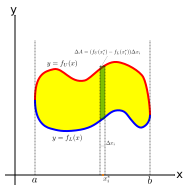
\includegraphics[width = 0.5\textwidth]{area_by_single_integral}
} & \parbox{0.5\textwidth}{
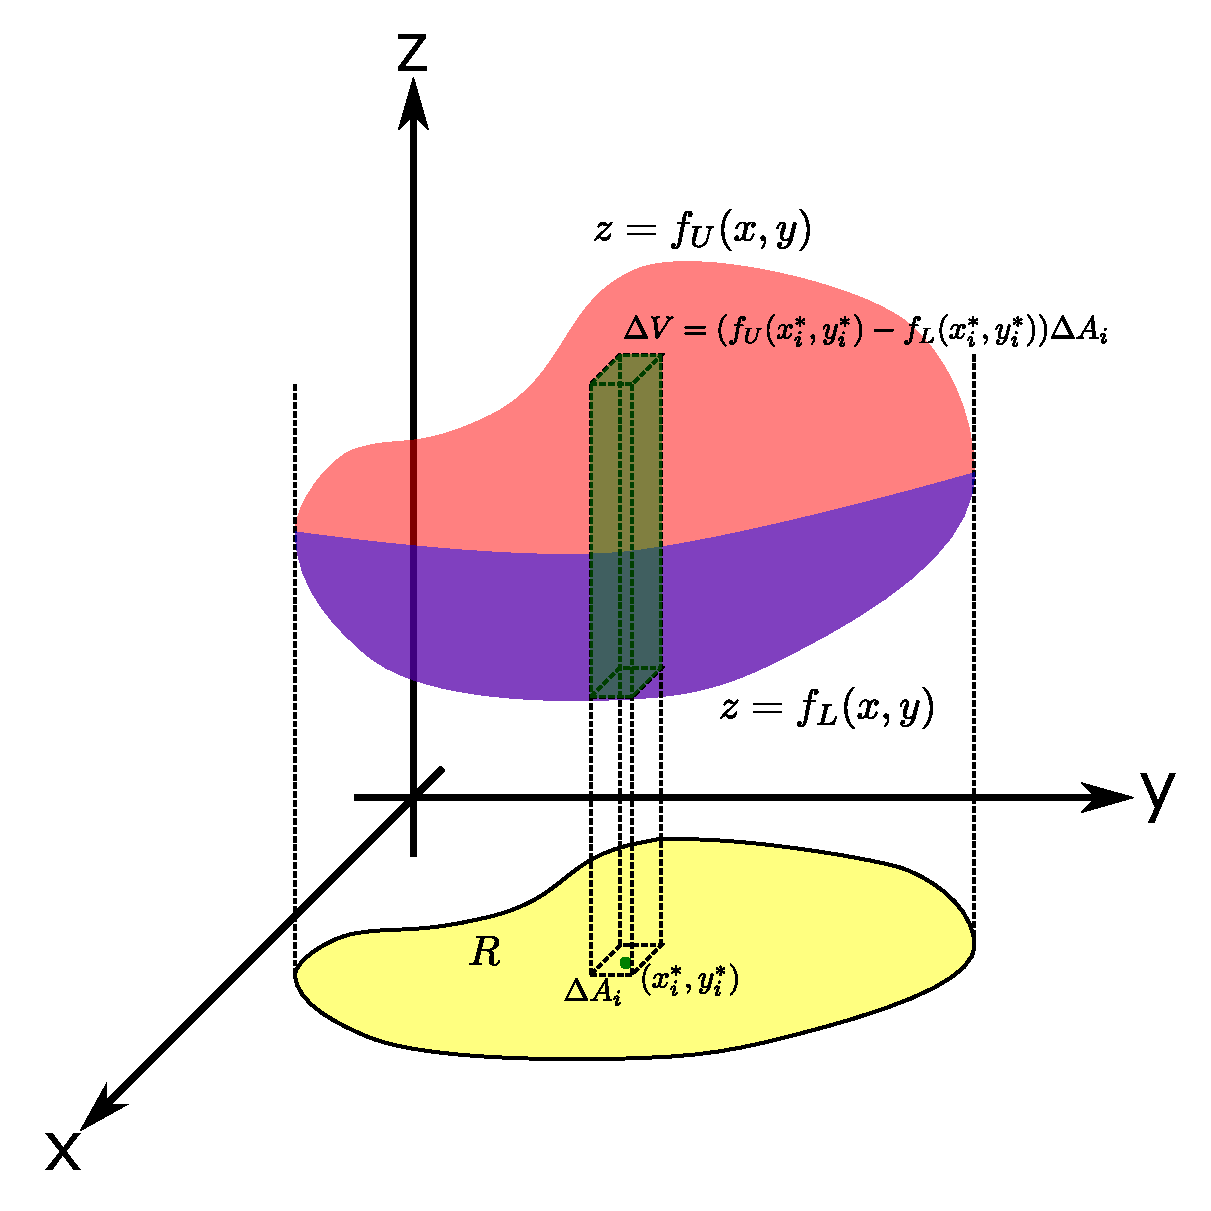
\includegraphics[width = 0.5\textwidth]{volume_by_double_integral}
}
\end{tabular}

If the ``horizontal" plane uses polar coordinates, then the double integral uses polar coordinates.

\vspace{5mm}

\textbf{Examples:}

\begin{itemize}
%%%%%%%%%%%%%%%%
\item ~~\\

\begin{tabular}{cc}
\parbox{0.5\textwidth}{
Consider the tetrahedron \(\Omega\) in the image on the right. Variables \(a\), \(b\), and \(c\) are fixed arbitrary constants. The volume of \(\Omega\) is sought. A quantification of \(\Omega\) can be derived as follows. 

The bounds on \(x\) are \(0\) and \(a\). 

The lower bound on \(y\) is \(0\), while the upper bound on \(y\) is line \(AB\). In the \(xy\) plane, the equation of line \(AB\) is: 
\begin{align*}
y - 0 = \frac{0 - b}{a - 0}(x - a) \iff y = b - \frac{b}{a}x
\end{align*}
The bounds on \(y\) as functions of \(x\) are \(0\) and \(b - \frac{b}{a}x\). 

The lower bound on \(z\) is \(0\), while the upper bound on \(z\) is the plane that passes through the points \(A\), \(B\), and \(C\). The equation of this plane can be derived as follows. A vector \(\mathbf{n}\) that is perpendicular to the plane is:
\[\mathbf{n} = \overrightarrow{AB} \times \overrightarrow{AC} = \begin{bmatrix} -a \\ b \\ 0 \end{bmatrix} \times \begin{bmatrix} -a \\ 0 \\ c \end{bmatrix} = \begin{bmatrix} bc - 0 \\ 0 - (-ac) \\ 0 - (-ab) \end{bmatrix} = \begin{bmatrix} bc \\ ac \\ ab \end{bmatrix}\]
} & \parbox{0.5\textwidth}{
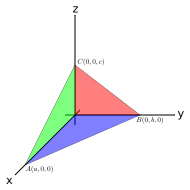
\includegraphics[width = 0.5\textwidth]{tetrahedron}
}
\end{tabular}

The equation of the plane is: 
\[\mathbf{n} \bullet \begin{bmatrix} x \\ y \\ z \end{bmatrix} = \mathbf{n} \bullet \begin{bmatrix} a \\ 0 \\ 0 \end{bmatrix} 
\iff bc x + ac y + ab z = abc \iff \frac{x}{a} + \frac{y}{b} + \frac{z}{c} = 1\]
Solving this equation for \(z\) yields \(z = c - \frac{c}{a}x - \frac{c}{b}y\). 
The bounds on \(z\) as functions of \(x\) and \(y\) are \(0\) and \(c - \frac{c}{a}x - \frac{c}{b}y\).  

The tetrahedron is:
\[\Omega = \left\{(x,y,z) \middle| 0 \leq x \leq a \;\&\; 0 \leq y \leq b - \frac{b}{a}x \;\&\; 0 \leq z \leq c - \frac{c}{a}x - \frac{c}{b}y \right\}\]

The volume of the tetrahedron is the triple integral of \(1\) over \(\Omega\): 

\begin{align*}
\iiint_{\Omega} dV = & 
\int_{x = 0}^a \left(\int_{y = 0}^{b - \frac{b}{a}x} \left(\int_{z = 0}^{c - \frac{c}{a}x - \frac{c}{b}y} dz\right)dy\right)dx 
= \int_{x = 0}^a \left(\int_{y = 0}^{b - \frac{b}{a}x} \left(c - \frac{c}{a}x - \frac{c}{b}y\right)dy\right)dx \\  
= & \int_{x = 0}^a \left(cy - \frac{c}{a}xy - \frac{c}{2b}y^2\right)\bigg|_{y = 0}^{b - \frac{b}{a}x} dx \\ 
= & \int_{x = 0}^a \left(c\left(b - \frac{b}{a}x\right) - \frac{c}{a}x\left(b - \frac{b}{a}x\right) - \frac{c}{2b}\left(b - \frac{b}{a}x\right)^2\right)dx \\ 
= & \int_{x = 0}^a \left(\left(bc - \frac{bc}{a}x\right) + \left(-\frac{bc}{a}x + \frac{bc}{a^2}x^2\right) - \frac{c}{2b}\left(b^2 - \frac{2b^2}{a}x + \frac{b^2}{a^2}x^2\right)\right)dx \\   
= & \int_{x = 0}^a \left(\left(bc - \frac{2bc}{a}x + \frac{bc}{a^2}x^2\right) + \left(-\frac{bc}{2} + \frac{bc}{a}x - \frac{bc}{2a^2}x^2\right)\right)dx \\   
= & \int_{x = 0}^a \left(\frac{bc}{2} - \frac{bc}{a}x + \frac{bc}{2a^2}x^2\right)dx   
= \left(\frac{bc}{2}x - \frac{bc}{2a}x^2 + \frac{bc}{6a^2}x^3\right)\bigg|_{x = 0}^a \\ 
= & \frac{abc}{2} - \frac{abc}{2} + \frac{abc}{6} 
= \frac{abc}{6}
\end{align*}

%%%%%%%%%%%%%%%%
\item ~~\\ 

\begin{tabular}{cc}
\parbox{0.5\textwidth}{
Consider the solid \(\Omega\) that is bounded from below by the surface \(z = -1\), and is bounded from above by the surface \(z = x - 1\). Moreover, let the \((x,y)\) coordinates be confined to the triangle with the vertices \((0, 0)\), \((1, 0)\), and \((1, 1)\). The volume of \(\Omega\) is sought. \(\Omega\) is depicted on the right. The region \(R\) that the \((x, y)\) coordinates are confined to can be quantified as follows: 

The bounds on \(x\) are \(0\) and \(1\), and the bounds on \(y\) are \(0\) and \(x\). The region \(R\) is:
\[R = \{(x,y) | 0 \leq x \leq 1 \;\&\; 0 \leq y \leq x\}\] 

\(\Omega\) is bounded from below and above respectively by the surfaces \(z = -1\) and \(z = x - 1\), so let \(f_L(x,y) = -1\) and \(f_U(x,y) = x - 1\). The volume of \(\Omega\) is derived below:
} & \parbox{0.5\textwidth}{
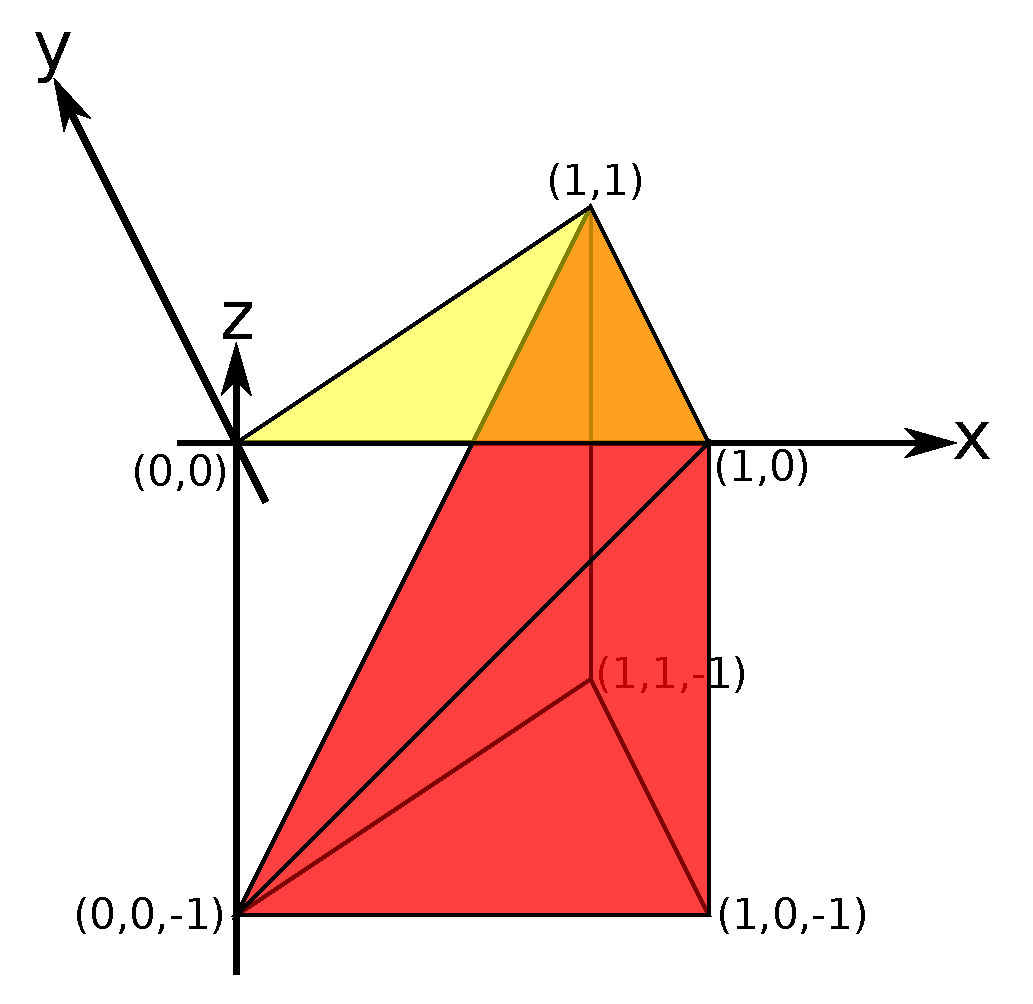
\includegraphics[width = 0.5\textwidth]{volume_example_1}
}
\end{tabular}

\begin{align*}
V = & \iint_R (f_U(x,y) - f_L(x,y))dA 
= \iint_R ((x-1) - (-1))dA 
= \iint_R x \cdot dA \\ 
= & \int_{x = 0}^1 \left(\int_{y = 0}^x x \cdot dy\right)dx
= \int_{x = 0}^1 xy \bigg|_{y = 0}^x dx 
= \int_{x = 0}^1 x^2 dx 
= \frac{1}{3}x^3\bigg|_{x=0}^1 
= \frac{1}{3}
\end{align*}

%%%%%%%%%%%%%%%%
\item ~~\\ 

\begin{tabular}{cc} 
\parbox{0.5\textwidth}{
Consider a sphere with a radius of \(a\). On the right, a sphere with a radius of \(a\) is centered on the origin. The \(x\) and \(y\) coordinates are confined to the circle \(R\) with a radius of \(a\) centered on \((0,0)\). This circle in polar coordinates is:
\[R = \{(r,\theta) | 0 \leq \theta \leq 2\pi \;\&\; 0 \leq r \leq a\}\]
The sphere is bounded from below by the surface 
\[z = -\sqrt{a^2 - r^2}\]
and is bounded from above by the surface 
\[z = \sqrt{a^2 - r^2}\]
\(r\) is the polar coordinate from \((r, \theta)\), the polar coordinate equivalent of the 2D Cartesian coordinate pair \((x,y)\). In essence \(r = \sqrt{x^2 + y^2}\). The 3D coordinate \(z\) has no impact on the value of \(r\), since the coordinates \((r, \theta)\) are coordinates of a point in the \(xy\) plane. 
} & \parbox{0.5\textwidth}{
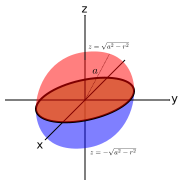
\includegraphics[width = 0.5\textwidth]{sphere_volume}
}
\end{tabular}

The volume of the sphere is 
\[\iint_R (f_U(r,\theta) - f_L(r,\theta))dA\]
where \(f_L(r,\theta) = -\sqrt{a^2 - r^2}\) and \(f_U(r,\theta) = \sqrt{a^2 - r^2}\). Note that this double integral is using polar coordinates.

\begin{align*}
V = & \iint_R (f_U(r,\theta) - f_L(r,\theta))dA 
= \iint_R (\sqrt{a^2 - r^2} - (-\sqrt{a^2 - r^2}))dA \\ 
= & \iint_R 2\sqrt{a^2 - r^2} \cdot dA   
= \int_{\theta = 0}^{2\pi} \left(\int_{r = 0}^a 2\sqrt{a^2 - r^2} \cdot r \cdot dr \right)d\theta 
= \int_{\theta = 0}^{2\pi} \left(\int_{r = 0}^a -\sqrt{a^2 - r^2} \cdot (-2rdr) \right)d\theta \\
= & \int_{\theta = 0}^{2\pi} -\frac{2}{3}(a^2 - r^2)^{3/2}\Big|_{r = 0}^a d\theta  
= \int_{\theta = 0}^{2\pi} (0 - (-\frac{2}{3}(a^2)^{3/2})) d\theta 
= \int_{\theta = 0}^{2\pi} \frac{2}{3}a^3 d\theta   
= \frac{2}{3}a^3\theta\bigg|_{\theta = 0}^{2\pi} 
= \frac{4}{3}\pi a^3
\end{align*}

%%%%%%%%%%%%%%%%
\item ~~\\ 
Consider the volume \(\Omega\) between the paraboloid \(x = 2y^2 + 2z^2 - 7\) and the plane \(x = 1\). The intersection between these surfaces is occurs when
\[2y^2 + 2z^2 - 7 = 1 \iff 2y^2 + 2z^2 = 8 \iff y^2 + z^2 = 4 \iff \sqrt{y^2 + z^2} = 4\]

\begin{tabular}{cc} 
\parbox{0.5\textwidth}{
The intersection is the circle with a radius of \(2\) that is centered on the point \((1, 0, 0)\) and is parallel to the \(yz\) plane. 
The \(y\) and \(z\) coordinates are confined to the circle \(R\) with a radius of \(2\) centered on the point \((0,0)\) in a \(yz\) coordinate system. This circle in polar coordinates is:
\[R = \{(r,\theta) | 0 \leq \theta \leq 2\pi \;\&\; 0 \leq r \leq 2\}\]
\(r\) is the polar coordinate from \((r, \theta)\), the polar coordinate equivalent of the 2D Cartesian coordinate pair \((y,z)\). In essence \(r = \sqrt{y^2 + z^2}\). The 3D coordinate \(x\) has no impact on the value of \(r\), since the coordinates \((r, \theta)\) are coordinates of a point in the \(yz\) plane. 
\(\Omega\) is bounded from ``below" by the paraboloid 
\[x = 2y^2 + 2z^2 - 7 = 2r^2 - 7\]
and is bounded from ``above" by the plane 
\[x = 1\]
} & \parbox{0.5\textwidth}{
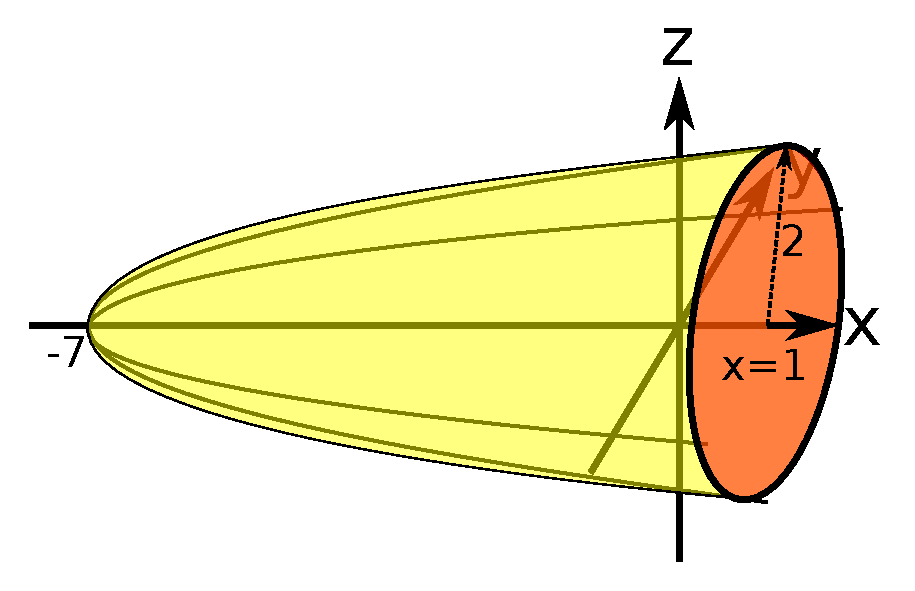
\includegraphics[width = 0.5\textwidth]{volume_example_2}
}
\end{tabular}

The volume of \(\Omega\) is: 
\[\iint_R (f_U(r,\theta) - f_L(r,\theta))dA\]
where \(f_L(r,\theta) = 2r^2 - 7\) and \(f_U(r,\theta) = 1\). Note that this double integral is using polar coordinates.

\begin{align*}
V = & \iint_R (f_U(r,\theta) - f_L(r,\theta))dA 
= \iint_R (1 - (2r^2 - 7))dA \\ 
= & \iint_R (8 - 2r^2)dA   
= \int_{\theta = 0}^{2\pi} \left(\int_{r = 0}^2 (8 - 2r^2) \cdot r \cdot dr \right)d\theta 
= \int_{\theta = 0}^{2\pi} \left(\int_{r = 0}^2 (8r - 2r^3) \right)d\theta \\
= & \int_{\theta = 0}^{2\pi} (4r^2 - \frac{1}{2}r^4)\Big|_{r = 0}^2 d\theta  
= \int_{\theta = 0}^{2\pi} ((16 - 8) - 0) d\theta 
= \int_{\theta = 0}^{2\pi} 8 d\theta   
= 8\theta\bigg|_{\theta = 0}^{2\pi} 
= 16\pi
\end{align*}

\end{itemize}






\section*{Average Value}

The ``average" value of a single variable function \(f(x)\) over the interval \([a, b]\) is:
\[f_{\text{ave}} = \frac{1}{b-a}\int_{x=a}^b f(x)dx\]

The ``average" value of a two variable function \(f(x,y)\) over the 2D region \(R\) is:
\[f_{\text{ave}} = \frac{1}{\text{area of \(R\)}}\iint_R f(x,y)dA\]

The ``average" value of a three variable function \(f(x,y,z)\) over the 3D region \(\Omega\) is:
\[f_{\text{ave}} = \frac{1}{\text{volume of \(\Omega\)}}\iiint_{\Omega} f(x,y,z)dV\]

\textbf{Examples:}
\begin{itemize}
%%%%%%%%%%%%%%%%%%%%%%%%%%
\item 
Consider the two variable function: 
\[f(x,y) = 2xy - x - \frac{7}{2}y + \frac{19}{2}\]
The average value of \(f(x,y)\) over the rectangle:
\[R = [0, 2] \times [-1, 3] = \{(x,y) | 0 \leq x \leq 2 \;\&\; -1 \leq y \leq 3\}\]
will be computed.

The area of the rectangle \(R\) is:
\[\text{area}(R) = 2 \cdot 4 = 8\]

The double integral of \(f(x,y)\) over \(R\) is:
\begin{align*}
& \iint_R f(x, y)dA  
= \iint_R \left(2xy - x - \frac{7}{2}y + \frac{19}{2}\right)dA 
= \int_{x = 0}^2 \left(\int_{y = -1}^3 \left(2xy - x - \frac{7}{2}y + \frac{19}{2}\right)dy\right)dx \\   
& = \int_{x = 0}^2 \left(xy^2 - xy - \frac{7}{4}y^2 + \frac{19}{2}y\right)\bigg|_{y = -1}^3 dx 
= \int_{x = 0}^2 \left(\left(9x - 3x - \frac{63}{4} + \frac{57}{2}\right) - \left(x + x - \frac{7}{4} - \frac{19}{2}\right)\right) dx \\  
& = \int_{x = 0}^2 \left(6x - 2x - \frac{56}{4} + \frac{76}{2}\right)dx 
= \int_{x = 0}^2 \left(4x - 14 + 38\right)dx 
= \int_{x = 0}^2 \left(4x + 24\right)dx  
= (2x^2 + 24x)\Big|_{x=0}^2 \\
& = (8 + 48) - 0 = 56
\end{align*}

The average value of \(f(x,y)\) over the rectangle \(R\) is:
\[f_{\text{ave}} = \frac{\iint_R f(x, y)dA}{\text{area}(R)} = \frac{56}{8} = 7\]
\end{itemize}






\end{document}












